%
% analytisch.tex
%
% (c) 2021 Prof Dr Andreas Müller, OST Ostschweizer Fachhochschule
%
\section{Analytische Funktionen
\label{buch:funktionentheorie:section:analytisch}}
\rhead{Analytische Funktionen}
Holomorphe Funktionen zeichnen sich dadurch aus, dass sie auch immer
eine konvergente Reihenentwicklung haben, sie sind also analytisch.

\subsection{Definition}
\index{Taylor-Reihe}%
\index{Exponentialfunktion}%
Die Taylor-Reihenentwicklung der Exponentialfunktion ermöglicht deren
effiziente Berechnung.
Es ist aber nicht selbstverständlich, dass die Taylor-Reihe überhaupt
gegen die Funktion konvergiert, aus deren Ableitungen sie gebildet
worden ist, wie das folgende Beispiel illustriert.

\begin{figure}
\centering
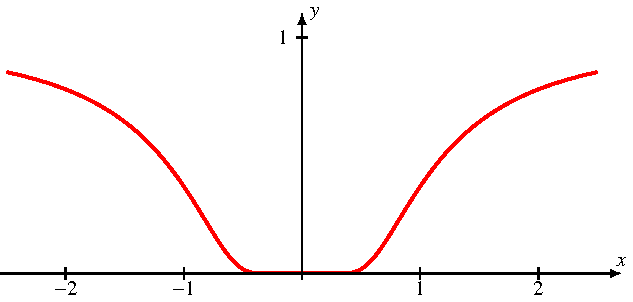
\includegraphics{chapters/080-funktionentheorie/images/nonanalytic.pdf}
\caption{Beispiel einer beliebig oft stetig differenzierbaren Funktion,
deren Ableitungen in $x=0$ alle verschwinden.
Die zugehörige Taylor-Reihe ist die Nullfunktion, sie hat nichts mit der
Funktion zu tun.
\label{buch:funktionentheorie:fig:nonanalytic}}
\end{figure}

\begin{beispiel}
Wir betrachten die Funktion
\[
f\colon \mathbb{R}\to\mathbb{R}
:
x \mapsto
\begin{cases}
e^{-1/x^2}&\qquad x\ne 0\\
0&\qquad x=0.
\end{cases}
\]
Der Graph $y=f(x)$ ist in Abbildung~\ref{buch:funktionentheorie:fig:nonanalytic}
dargestellt.

Die ersten zwei Ableitungen der Funktion $f$ sind
\begin{align*}
f'(x) &= \frac{2e^{-1/x^2}}{x^3} = \frac{2}{x^3}\cdot f(x)
\\
f''(x) &= \frac{(4-6x^2) e^{-1/x^2}}{x^6} = \frac{4-6x^2}{x^6}\cdot f(x)
\\
&\dots
\end{align*}
Man kann vermuten, dass alle
Ableitungen Funktionen der Form
\begin{equation}
F(x) = \frac{p(x)}{x^n} \cdot f(x),
\label{buch:funktionentheorie:eqn:nonanalytic:form}
\end{equation}
sind,
wobei $p(x)$ ein Polynom ist.
Leitet man eine solche Funktion nach $x$ ab, erhält man
\begin{align*}
\frac{d}{dx} F(x)
&=
\frac{\frac{d}{dx}(p(x)f(x)) x^n - nx^{n-1}p(x)f(x)}{x^{2n}}
\\
&=
\frac{p'(x)f(x) + p(x)f'(x) - nx^{n-1}p(x)f(x)}{x^{2n}} 
\\
&=
\frac{p'(x) + p(x)(2/x^3) - nx^{n-1}p(x)}{x^{2n}} \cdot f(x)
\\
&=
\frac{x^3p'(x)+2p(x)-nx^{n-1}p(x)}{x^{2n+3}}\cdot f(x).
\end{align*}
Dies ist wieder eine Funktion der
Form~\eqref{buch:funktionentheorie:eqn:nonanalytic:form}.

Der Faktor $f(x)=e^{-1/x^2}$ von $F(x)$ geht für $x\to 0$ exponentiell
schnell gegen $0$, schneller als der Nenner $x^n$ gegen $0$ gehen
kann. 
Der Grenzwert $x\to 0$ einer Funktion der 
Form~\eqref{buch:funktionentheorie:eqn:nonanalytic:form}
ist daher immer
\[
\lim_{x\to 0}  F(x) =0.
\]
Damit ist gezeigt, dass alle Ableitungen $f^{(n)}(0)=0$ sind.
Die Taylorreihe von $f(x)$ ist daher die Nullfunktion.
\end{beispiel}

Die Klasse der Funktionen, die sich durch ihre Taylor-Reihe darstellen
lassen, zeichnet sich also durch besondere Eigenschaften aus, die in
der folgenden Definition zusammengefasst werden.

\index{analytisch in einem Punkt}%
\index{analytisch}%
\begin{definition}
Eine auf einem offenen Intervall $I\subset \mathbb {R}$ definierte Funktion
$f\colon U\to\mathbb{R}$ heisst {\em analytisch im Punkt  $x_0\in I$}, wenn
es eine in einer Umgebung von $x_0$ konvergente Potenzreihe
\[
\sum_{k=0}^\infty a_k(x-x_0)^k = f(x)
\]
gibt.
Sie heisst {\em analytisch}, wenn sie analytisch ist in jedem Punkt von $I$.
\end{definition}

Es ist wohlbekannt aus der elementaren Theorie der Potenzreihen, dass
eine analytische Funktion beliebig oft differenzierbar ist und dass
die Potenzreihe im Punkt $x_0$ die Taylor-Reihe sein muss.
Ausserdem sidn Summen, Differenzen und Produkte von analytischen Funktionen
wieder analytisch.

Für eine komplexe Funktion lässt sich der Begriff der
analytischen Funktion genau gleich definieren.

\begin{definition}
Eine in einer offenen Teilmenge $U\subset \mathbb{C}$ definierte Funktion
$f\colon U\to\mathbb{C}$ heisst {\em analytisch im Punkt $z_0\in U$}, wenn
es eine in einer Umgebung von $z_0$ konvergente Potenzreihe
\[
\sum_{k=0}^\infty a_k(z-z_0)^k = f(z)
\]
gibt.
Sie heisst {\em analytisch}, wenn sie analytisch ist in jedem Punkt von $U$.
\end{definition}

Die Verwendung einer offenen Teilmenge $U\subset\mathbb{C}$ ist wesentlich,
denn die Funktion $f\colon z\mapsto \overline{z}$ kann in jedem Punkt
$x_0\in\mathbb{R}$
der reellen Achse $\mathbb{R}\subset\mathbb{C}$ durch die Potenzreihe 
$f(x) = x_0 + (x-x_0)$ dargestellt werden.
Es gibt aber keine Potenzreihe, die $f(z)$ in einer offenen Teilmenge
von $\mathbb{C}$ gegen $f(z)=\overline{z}$ konvergiert.

%
% Der Konvergenzradius einer Potenzreihe
%
\subsection{Konvergenzradius
\label{buch:funktionentheorie:subsection:konvergenzradius}}

% XXX auf dem Rand des Konvergenzkreises gibt es immer eine Singularität


